\section{A conformal lens with a uniform boundary coordinate}\label{sec:lens}

We construct a conformal image of the disk whose boundary has a uniformly
distributed imaginary coordinate. This law will turn complex feasibility
probabilities into real volumes. The horizontal half-width has further
roles: strict curvature will make additional boundary equalities have
probability zero,
while concavity will extend feasibility from polar vertices to their
convex hull. Its endpoint scaling will enter the equality argument near
the apex of the lifted body.
The map is a rotation of the uniform-distribution example in
Gross's conformal Skorokhod embedding~\cite[Section~3.2]{Gross}; we prove
all its required properties directly.

Write $\mathbb D=\{z\in\mathbb C:|z|<1\}$ and define
\begin{equation}\label{eq:lens-map}
 F(z)=\frac8{\pi^2}\sum_{j=0}^{\infty}
             \frac{(-1)^jz^{2j+1}}{(2j+1)^2}.
\end{equation}
The series converges uniformly on $\overline{\mathbb D}$.

\begin{lemma}[The planar lens]\label{lem:planar-lens}
The function $F$ is a biholomorphism from $\mathbb D$ onto a bounded
convex domain $D$, with inverse $g$, and $F'(0)=8/\pi^2$.
There is a continuous even function $\lambda:[-1,1]\to[0,\infty)$,
positive on $(-1,1)$ and zero at $\pm1$, such that
\begin{equation}\label{eq:lens-domain}
 \overline D=\{v+it:|t|\leq1,\ |v|\leq\lambda(t)\}.
\end{equation}
The function $\lambda$ is smooth on $(-1,1)$ and satisfies
\begin{equation}\label{eq:lens-width-curvature}
 \lambda'(t)=-\frac2\pi
       \operatorname{arctanh}\!\left(\sin\frac{\pi t}{2}\right),
 \qquad
 \lambda''(t)=-\sec\frac{\pi t}{2}<0.
\end{equation}
If $\Theta$ is uniform on $[0,2\pi)$, then
\begin{equation}\label{eq:lens-boundary-law}
 F(e^{i\Theta})\ \stackrel{\mathrm{law}}{=}\
 \varepsilon\lambda(T)+iT,
\end{equation}
where $T$ is uniform on $[-1,1]$ and $\varepsilon$ is an independent
uniform sign.
\end{lemma}

\begin{proof}
The map is odd and commutes with conjugation. Put
\[
 w=\arctan z=\frac1{2i}\log\frac{1+iz}{1-iz},\qquad z\in\mathbb D.
\]
The fraction inside the logarithm lies in the right half-plane, where
we use the principal logarithm. Thus $|\Re w|<\pi/4$, $\tan w=z$,
and $w=0$ only when $z=0$. Differentiating the series gives
\begin{equation}\label{eq:lens-derivatives}
 F'(z)=\frac8{\pi^2}\frac wz,\qquad
 1+\frac{zF''(z)}{F'(z)}=\frac{\sin(2w)}{2w},
\end{equation}
with their limiting values at zero. In particular $F'$ has no zeros.
For $w=a+ib\ne0$, the real part of the last expression is
\[
 \frac{a\sin(2a)\cosh(2b)+b\cos(2a)\sinh(2b)}{2(a^2+b^2)}>0,
\]
since $|a|<\pi/4$; its value at zero is $1$.

Fix $0<r<1$ and put $\gamma_r(\theta)=F(re^{i\theta})$.
This curve is regular, and its tangent angle $\beta$ satisfies
\[
 \beta'(\theta)=\Re\!\left(1+\frac{zF''(z)}{F'(z)}\right)>0,
 \qquad \beta(\theta+2\pi)=\beta(\theta)+2\pi.
\]
The second identity uses the zero-free derivative in the disk.
At a fixed parameter $\theta_0$, project the curve onto its right unit
normal there. The derivative of this projection has the sign of
$-\sin(\beta(\theta)-\beta(\theta_0))$. It is negative until the tangent
has turned through $\pi$, and positive thereafter, until the curve
returns to $\theta_0$. Hence the projection has its unique maximum at
$\theta_0$. This proves simplicity and shows that every point of the
curve is the unique supporting point of its convex hull in the
corresponding normal direction. All normal directions occur, so the
curve is the boundary of that convex hull and is positively oriented.
The harmonic maximum principle for these supporting projections places
$F(r\mathbb D)$ strictly inside the curve. The argument principle then
gives exactly one preimage for every point inside and none outside.
Thus $F$ maps $r\mathbb D$ biholomorphically onto its bounded convex
interior $D_r$.

As $r$ increases, these domains exhaust $D=F(\mathbb D)$. Consequently
$F$ is univalent on $\mathbb D$, $D$ is convex, and its inverse $g$ is
holomorphic. For each $0<r<1$, continuity also gives
$\overline{D_r}=F(r\overline{\mathbb D})\subset D$.
Continuity on the closed disk gives boundedness and
$\overline D=F(\overline{\mathbb D})$. No boundary value $F(\zeta)$,
$|\zeta|=1$, lies in $D$: otherwise continuity of $g$ there and
$g(F(r\zeta))=r\zeta$ would give $g(F(\zeta))=\zeta\notin\mathbb D$.
It follows that $\partial D=F(\partial\mathbb D)$.

We now compute this boundary. On the right semicircle,
$z=e^{is}$ with $-\pi/2<s<\pi/2$, one has
\[
 \frac{1+iz}{1-iz}=\frac{i\cos s}{1+\sin s},\qquad
 \Re w=\frac\pi4,\qquad
 \Im w=\frac12\operatorname{arctanh}(\sin s).
\]
The formulas for $w$ and $F'$ extend analytically across each compact
subarc, so we may differentiate the boundary values. Writing
$F(e^{is})=v(s)+it(s)$ gives
\[
 t'(s)=\frac2\pi,\qquad
 v'(s)=-\frac4{\pi^2}\operatorname{arctanh}(\sin s).
\]
Since $t(0)=0$, we have $t(s)=2s/\pi$. Define
$\lambda(t)=v(\pi t/2)$ and extend it to $[-1,1]$ by continuity.
Conjugation makes $\lambda$ even. The values $F(\pm i)$ are purely
imaginary by the series, so $\lambda(\pm1)=0$. Differentiation gives
\eqref{eq:lens-width-curvature}; strict concavity and the endpoint
values then give positivity in the interior.
Oddness and conjugation show that the other semicircle traces the graph
$v=-\lambda(t)$. These two graphs give \eqref{eq:lens-domain}.
On either semicircle the imaginary coordinate traverses $[-1,1]$
at constant absolute speed $2/\pi$. Each semicircle has probability
$1/2$, which proves \eqref{eq:lens-boundary-law}.
\end{proof}

Figure~\ref{fig:lens-boundary-law} illustrates the coordinate law.

\begin{figure}[htbp]
\centering
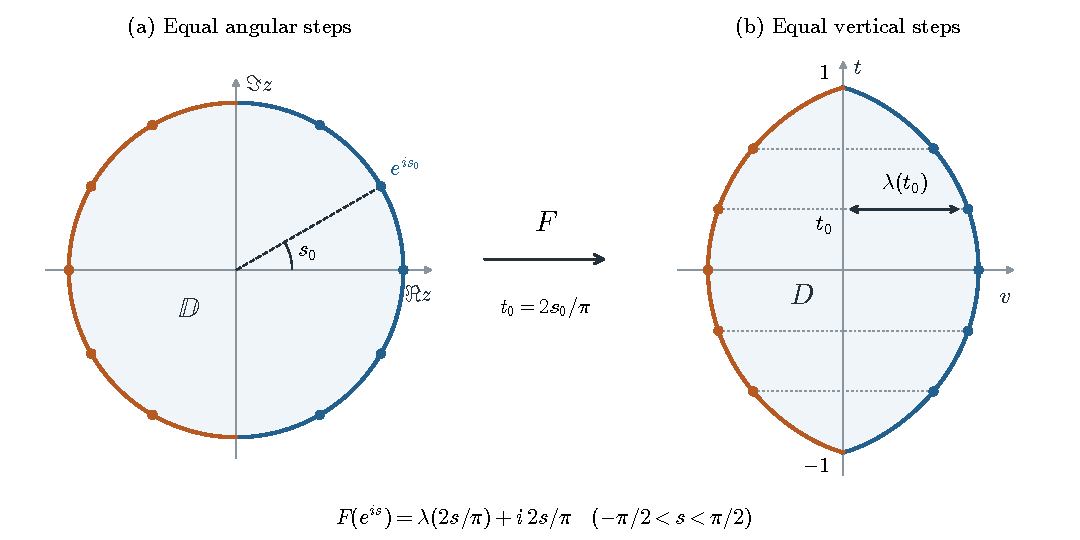
\includegraphics[width=\textwidth]{figures/lens-boundary-law.pdf}
\caption{The conformal lens and its boundary coordinate. Equally spaced
angles on either semicircle give equally spaced imaginary coordinates
on the corresponding boundary branch. On the right semicircle,
$F(e^{is})=\lambda(2s/\pi)+2is/\pi$; reflection gives the left branch.
Thus a uniform angle gives a uniform coordinate in $[-1,1]$ and an
independent fair branch sign. The horizontal arrow marks the
half-width $\lambda(t_0)$, with $s_0=\pi/6$ and $t_0=1/3$.}
\label{fig:lens-boundary-law}
\end{figure}

The two boundary graphs are smooth away from $\pm i$ and have strictly
turning tangent directions by \eqref{eq:lens-width-curvature}. In
particular, a fixed tangent line direction occurs at only finitely many
parameters away from these two endpoints. The boundary has planar
Lebesgue measure zero, as is also immediate from its graph description.

\begin{lemma}[Endpoint scaling]\label{lem:lens-endpoint}
As $\eta\downarrow0$,
\begin{equation}\label{eq:lens-endpoint-asymptotic}
 \lambda(1-\eta)=\frac2\pi\eta\log\frac1\eta+O(\eta).
\end{equation}
For every $0<a\leq b<\infty$,
\begin{equation}\label{eq:lens-endpoint-ratio}
 \sup_{a\leq c\leq b}
 \left|\frac{\lambda(1-\delta c)}{\lambda(1-\delta)}-c\right|
 \longrightarrow0\qquad(\delta\downarrow0).
\end{equation}
\end{lemma}

\begin{proof}
Equation~\eqref{eq:lens-width-curvature} and
$\operatorname{arctanh}(\cos x)=\log\cot(x/2)$ give
\[
 \lambda(1-\eta)=\frac2\pi\int_0^\eta
                  \log\cot\frac{\pi s}{4}\,ds.
\]
Here $\log\cot(\pi s/4)=\log(1/s)+O(1)$ uniformly as $s\downarrow0$.
Integration proves \eqref{eq:lens-endpoint-asymptotic}.
Writing $L=\log(1/\delta)$, the same uniform remainder gives
\[
 \frac{\lambda(1-\delta c)}{\lambda(1-\delta)}
 =c\,\frac{L-\log c+O(1)}{L+O(1)}
 =c+O_{a,b}(L^{-1})
\]
uniformly for $a\leq c\leq b$, which proves
\eqref{eq:lens-endpoint-ratio}.
\end{proof}
